\documentclass[12pt, a4paper]{article}

\usepackage[utf8]{inputenc}
\usepackage[russian]{babel}

\usepackage{graphicx}
\usepackage{amsfonts}
\usepackage{amsmath}
\usepackage{cmap}
\usepackage[hidelinks]{hyperref}
\usepackage{epstopdf}
\usepackage{cite}
\usepackage{indentfirst}
\usepackage{listings}
\usepackage{xcolor}
\usepackage{array}
\usepackage{float}

\usepackage[left=2cm,right=1cm,
top=2cm,bottom=2cm,bindingoffset=0cm]{geometry}

\graphicspath{{images/}}

\definecolor{codegreen}{rgb}{0,0.6,0}
\definecolor{codegray}{rgb}{0.5,0.5,0.5}
\definecolor{codepurple}{rgb}{0.58,0,0.82}
\definecolor{backcolour}{RGB}{185,185,185}

\lstdefinestyle{bashstyle}{
	language=bash,
	backgroundcolor=\color{backcolour},   
	commentstyle=\color{codegreen},
	keywordstyle=\color{magenta},
	numberstyle=\tiny\color{codegray},
	stringstyle=\color{codepurple},
	basicstyle=\ttfamily\footnotesize,
	breakatwhitespace=false,         
	breaklines=true,                 
	captionpos=b,                    
	keepspaces=true,                                  
	showspaces=false,                
	showstringspaces=false,
	showtabs=false,                  
	tabsize=2,
	emph={make, cmake, mkdir},
	emphstyle = {\color{magenta}},
}

\lstset{style=bashstyle}


\begin{document}
	
\thispagestyle{empty}

\begin{center}
	\ \vspace{-3cm}
	
	
\includegraphics[width=0.5\textwidth]{msu-eps-converted-to.pdf}\\
	{Московский государственный университет имени М. В. Ломоносова}\\
	Факультет вычислительной математики и кибернетики\\
	Кафедра вычислительных методов
	
	\vspace{6cm}
	
	{\Large \bfseries Построение разреженной матрицы и решение СЛАУ}
	
	\vspace{1cm}
	
	{\large Параллельные высокопроизводительные вычисления}
\end{center}

\vfill

\begin{flushright}
	\textbf{выполнил:}\\
	Петров Т.\,П. \\
	группа 504
\end{flushright}

\vfill

\begin{center}
	31 октября \\
	Москва, 2024
\end{center}

\enlargethispage{2\baselineskip}

\newpage

\tableofcontents

\newpage

\section{Описание задания и программной реализации}
\subsection{Краткое описание задания}

Необходимо реализовать многопоточную программу для решения систем линейных алгебраических уравнений (СЛАУ) на неструктурированной сетке с использованием OpenMP. Алгоритм должен состоять из нескольких этапов:

\begin{enumerate}
	\item Генерация графа сетки и его матричного представления – создание графа, связей элементов и его представление в разреженном формате CSR
	\item Заполнение матрицы СЛАУ – построение матрицы коэффициентов и вектора правой части с использованием тестовых формул
	\item Решение СЛАУ – реализация итерационного метода сопряженных градиентов для решения уравнения с поддержкой параллелизма
	\item Проверка производительности – измерение времени выполнения каждого этапа и анализ многопоточного ускорения и эффективности алгоритма
\end{enumerate}


\subsection{Краткое описание программной реализации}

...


\newpage

\section{Исследование производительности}

\subsection{Характеристики вычислительной системы}

\begin{center}
	\setlength{\tabcolsep}{30pt}
	\renewcommand{\arraystretch}{1.5}
	\begin{tabular}{ c|c|c } 
		 & PC & Polus \\ 
		\hline
		CPU  & i5-12400F & IBM POWER 8 \\ 
		Cores & 6 & 20 \\ 
		Threads & 2 & 8 \\
		TPP & 384 GFLOPS & 290 GFLOPS \\
		RAM & 2xDDR5-5600  & 4xDDR4-2400 \\
		BW & 89.6 GB/s & 307.2 GB/s \\
	\end{tabular}
\end{center}

Для того, чтобы собрать программу и скомпилировать все файлы, необходимо выполнить ряд следующих действий.

\begin{lstlisting}{bash}
	mkdir build && cd build
	cmake .. -DENABLE_TESTS=<On|Off>
	make -j 4
	cd ../bin
\end{lstlisting}

Для запуска на локальных системах достаточно указать количество нитей, а также все необходимые параметры:

\begin{lstlisting}{bash}
	OMP_NUM_THREADS=k ./a.out Nx Ny K1 K2
\end{lstlisting}

Для запуска на кластере, использующем систему очередей, запускается скрипт со следующими параметрами.

\begin{lstlisting}{bash}
	mpisubmit.pl params a.out -- a.out params
\end{lstlisting}

Однако желательно редактирование командного файла для запуска на заданных узлах и привязки к определенному сокету узла.

\begin{lstlisting}{bash}
	source /polusfs/setenv/setup.SMPI
	#BSUB -W 00:15
	#BSUB -o ../out/DotMeasure.%J.out
	#BSUB -e ../out/DotMeasure.%J.err
	#BSUB -m polus-c4-ib
	#BSUB -R affinity[core(10):distribute=pack(socket=1)]
	OMP_NUM_THREADS=1
	/polusfs/lsf/openmp/launchOpenMP.py ../DotMeasure
\end{lstlisting}


\subsection{Результаты измерений производительности}

\subsubsection{Последовательная производительность}

\begin{figure}[H]
	\center
	\begin{tabular}{cc}
		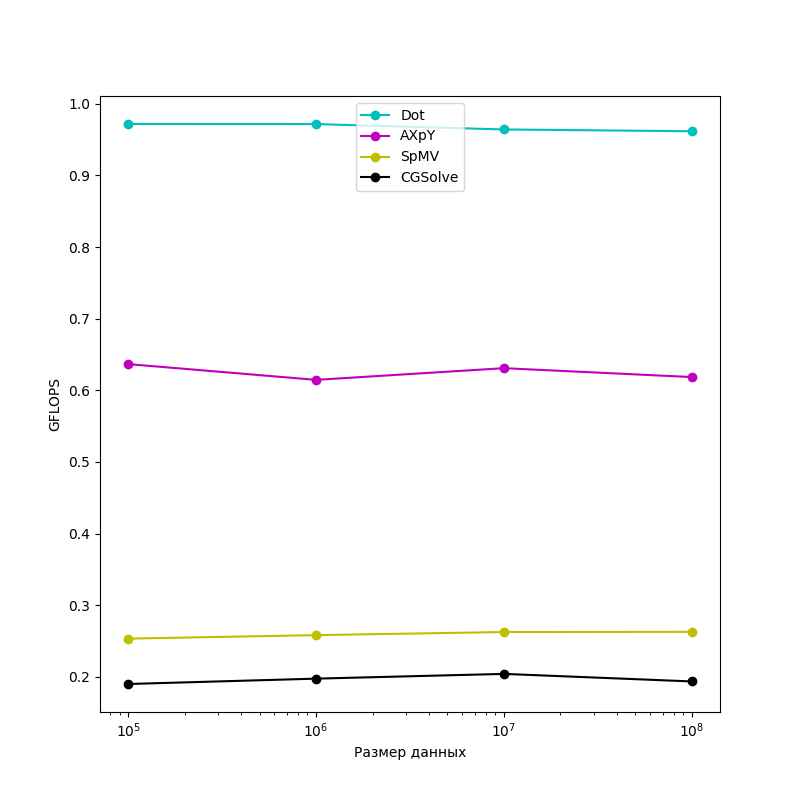
\includegraphics[width=85mm]{singlethread_pc} & 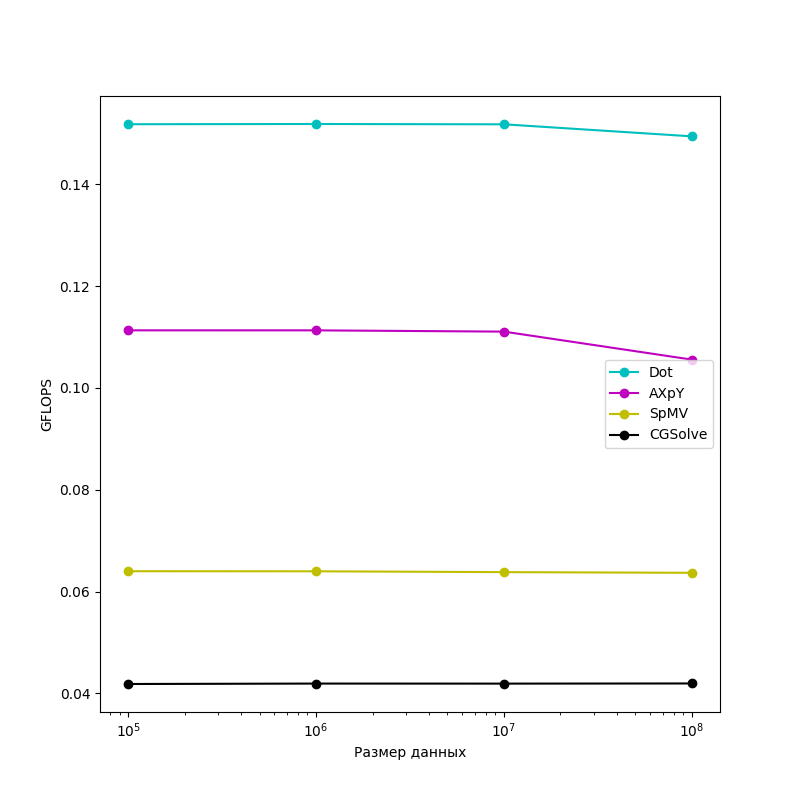
\includegraphics[width=85mm]{singlethread_polus} \\
		(а) PC & (б) Polus \\[6pt]
	\end{tabular}
	\caption{Зависимость производительности от размера входных данных} 
	\label{fig:singlethread_flops}
\end{figure}

\begin{figure}[H]
	\center
	\begin{tabular}{cc}
		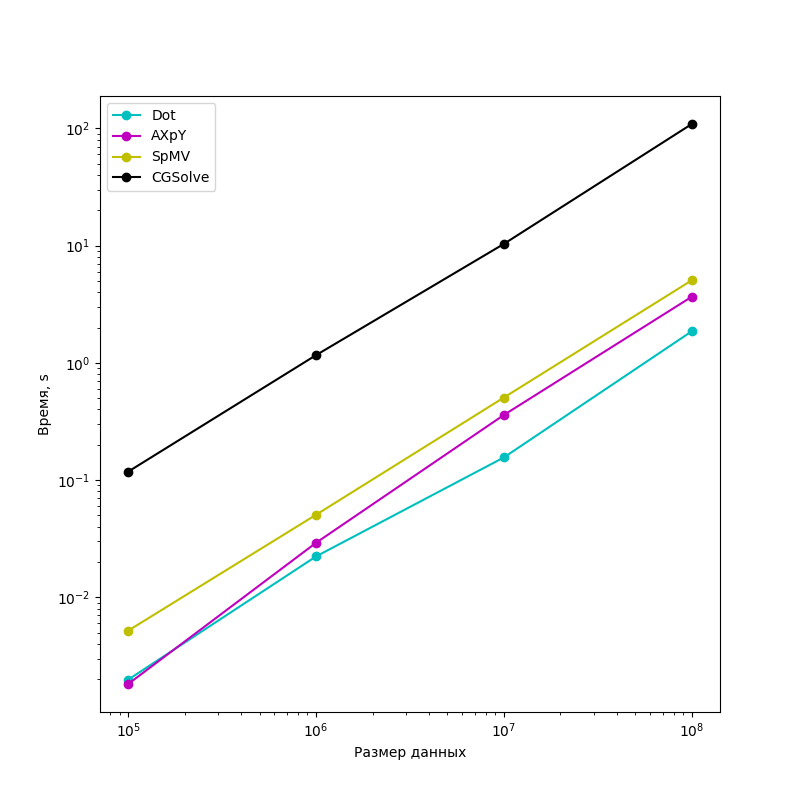
\includegraphics[width=85mm]{singlethread_time} & 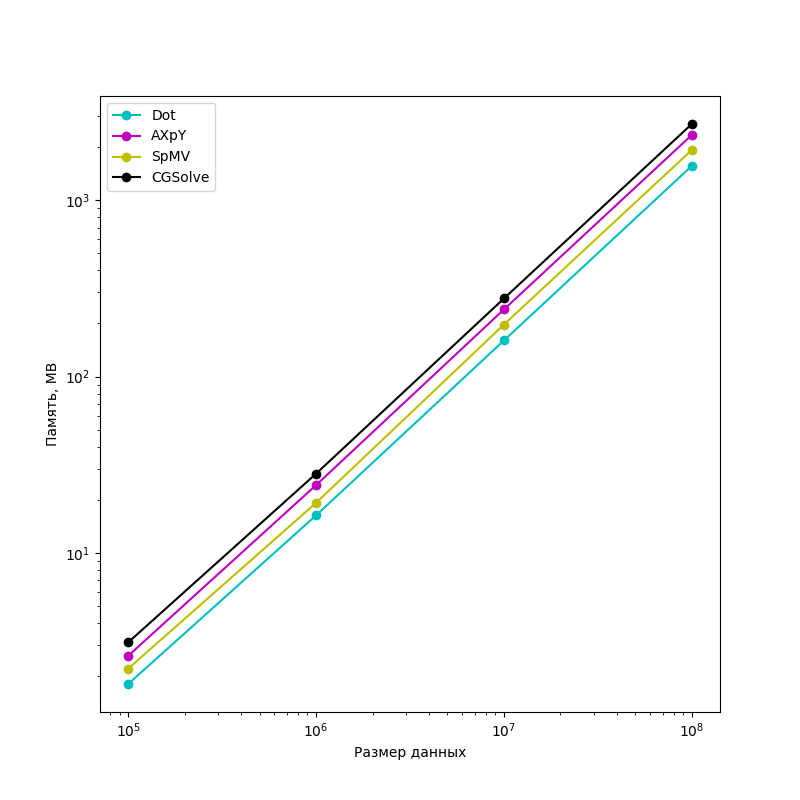
\includegraphics[width=85mm]{singlethread_memory} \\
		(а) & (б) \\[6pt]
	\end{tabular}
	\caption{Зависимость времени выполнения (а) и выделяемой памяти (б) в зависимости от размера входных данных}
	\label{fig:singlethread_time_memory}
\end{figure}

\subsubsection{Параллельное ускорение}

\begin{figure}[H]
	\center
	\begin{tabular}{cc}
		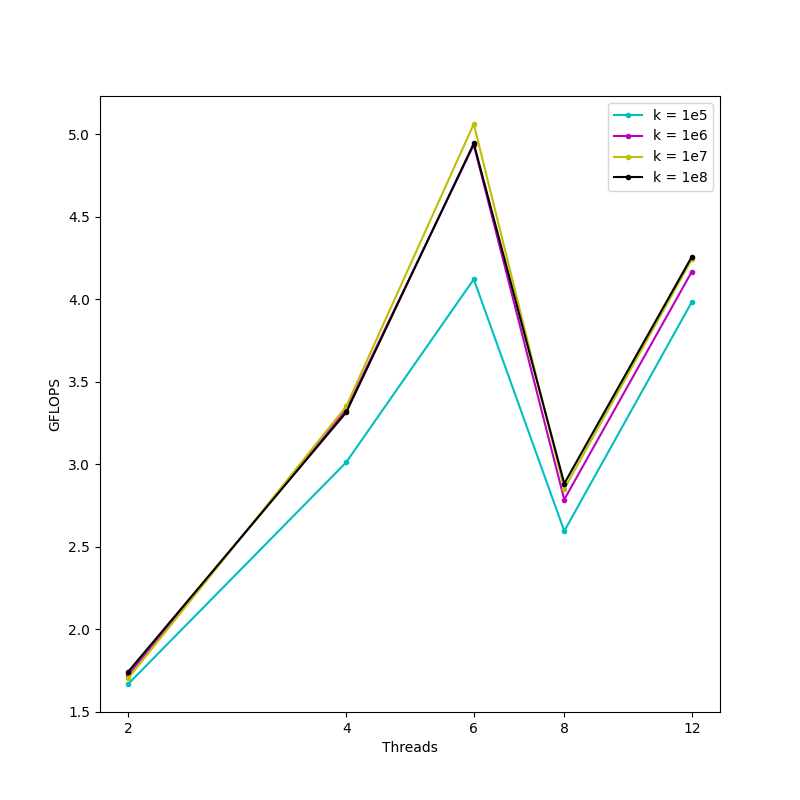
\includegraphics[width=85mm]{multithread_pc_dot} & 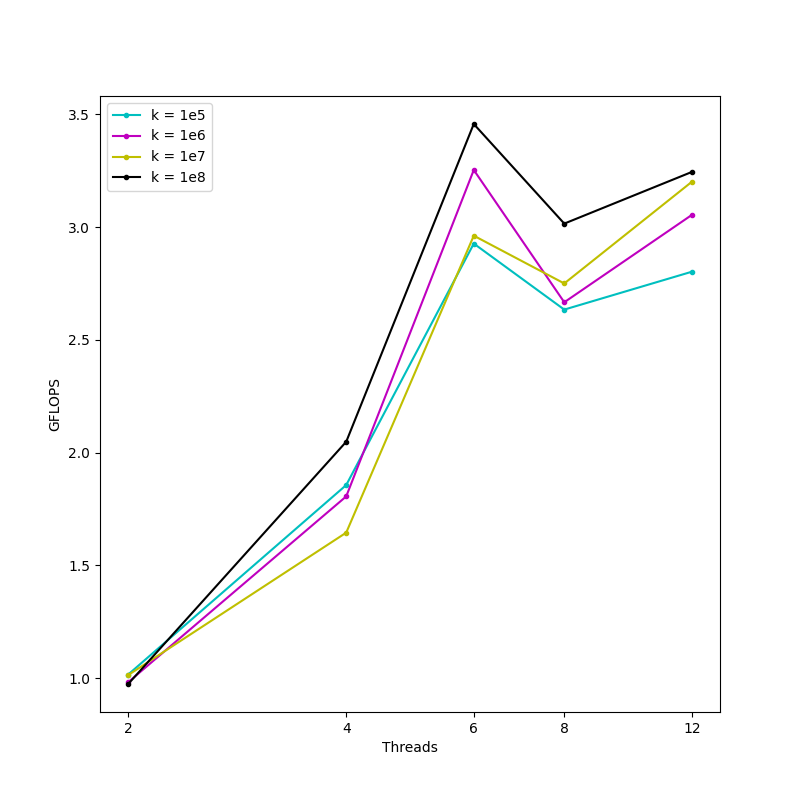
\includegraphics[width=85mm]{multithread_pc_axpy} \\
		(a) Dot & (б) AXpY \\
		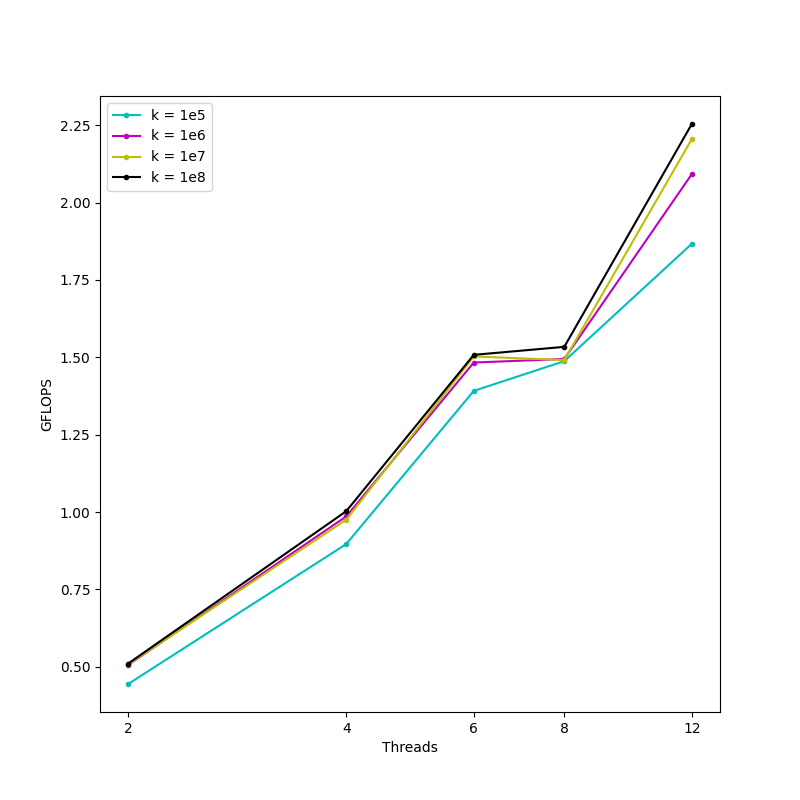
\includegraphics[width=85mm]{multithread_pc_spmv} & 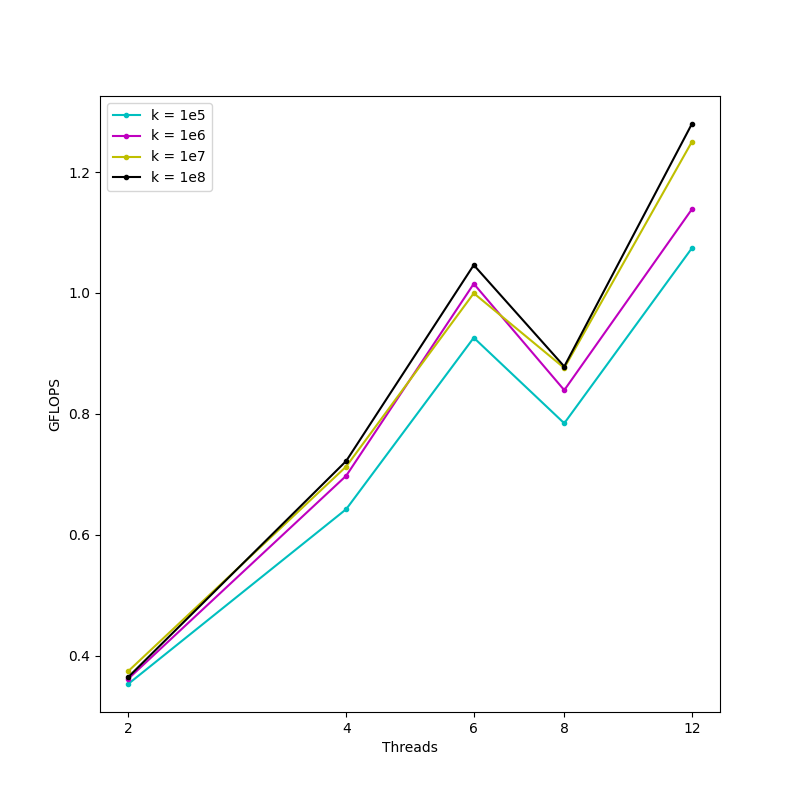
\includegraphics[width=85mm]{multithread_pc_cgsolver} \\
		(в) SpMV & (г) CGSolver \\[6pt]
	\end{tabular}
	\caption{Зависимость производительности от числа нитей (PC)}
	\label{fig:multithread_flops_pc} 
\end{figure}

\begin{figure}[H]
	\center
	\begin{tabular}{cc}
		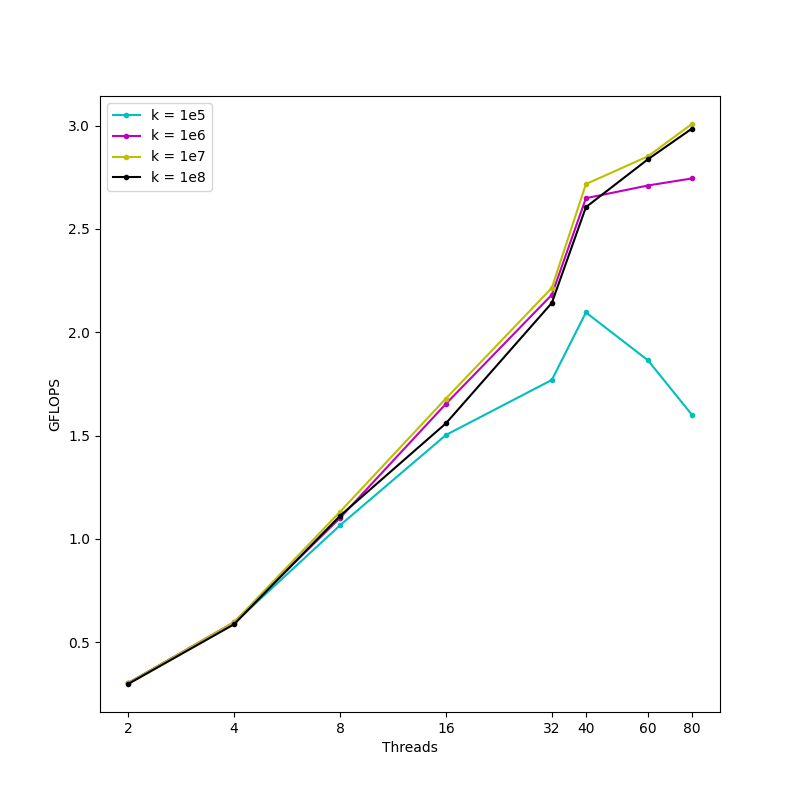
\includegraphics[width=85mm]{multithread_polus_dot} & 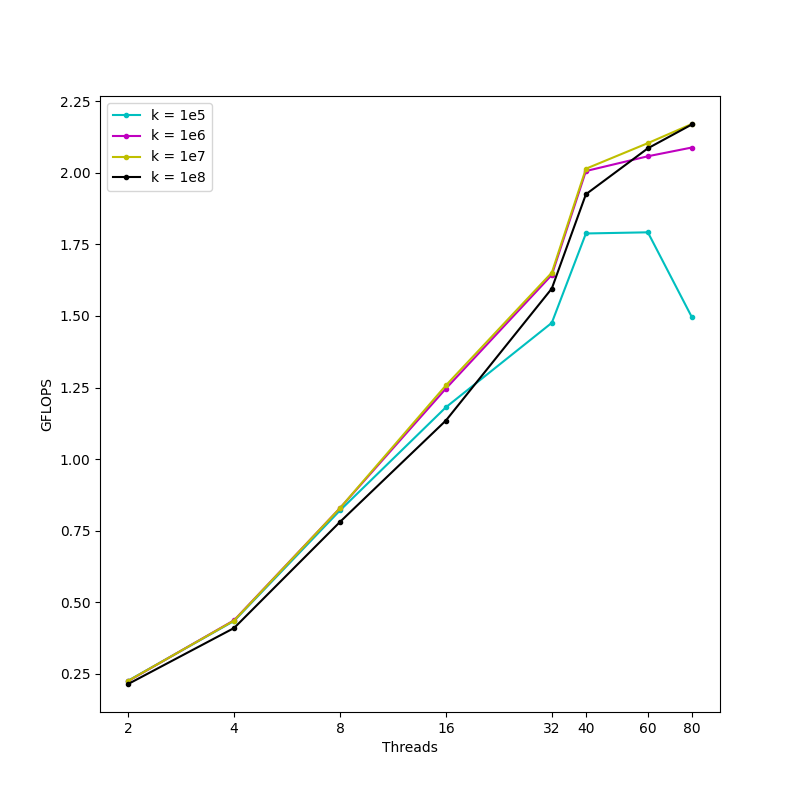
\includegraphics[width=85mm]{multithread_polus_axpy} \\
		(a) Dot & (б) AXpY \\
		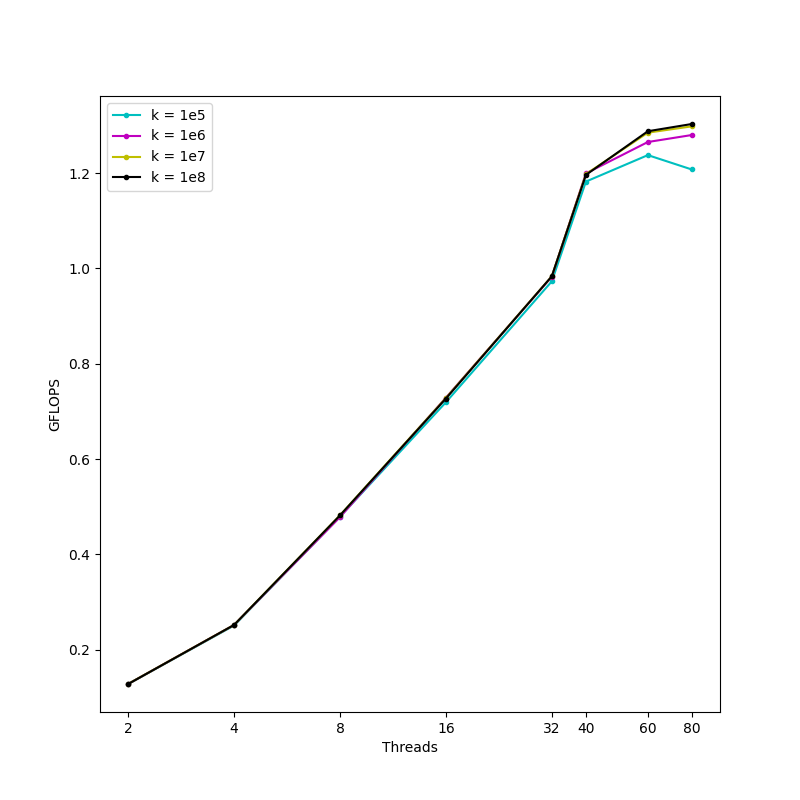
\includegraphics[width=85mm]{multithread_polus_spmv} & 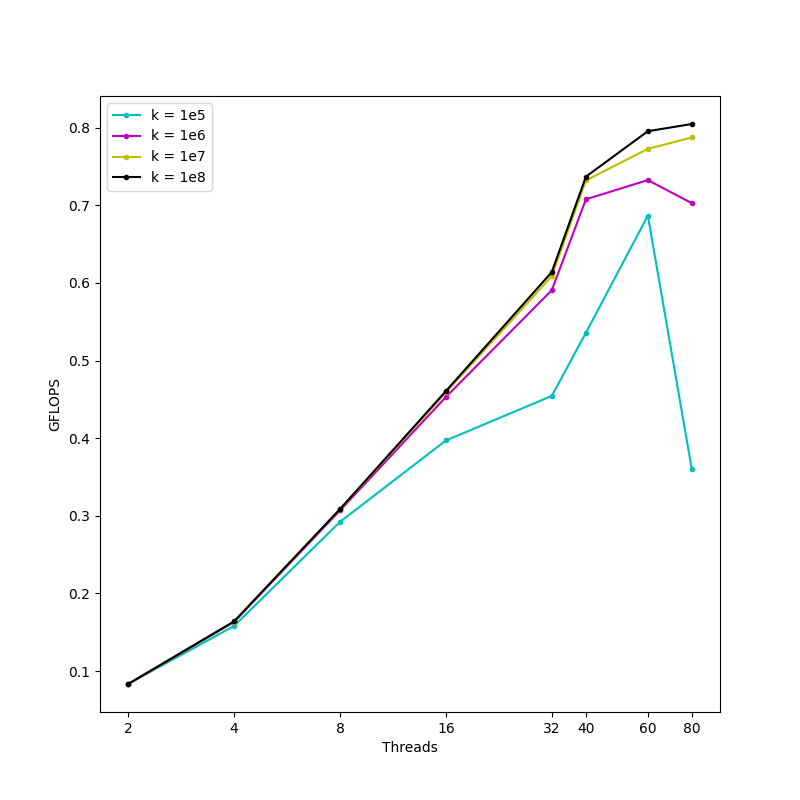
\includegraphics[width=85mm]{multithread_polus_cgsolver} \\
		(в) SpMV & (г) CGSolver \\[6pt]
	\end{tabular}
	\caption{Зависимость производительности от числа нитей на (Polus)}
	\label{fig:multithread_flops_polus} 
\end{figure}

\begin{figure}[H]
	\center
	\setlength{\tabcolsep}{10pt}
	\renewcommand{\arraystretch}{1.5}
	\begin{tabular}{|c|c|c|c|c|c|c|c|c|}
		\hline
		T & 2 & 4 & 8 & 16 & 32 & 40 & 64 & 80  \\
		\hline
		Dot &  &  &  &  &  &  &  &   \\
		\hline
		AXpY &  &  &  &  &  &  &  &   \\
		\hline
		SpMV &  &  &  &  &  &  &  &   \\
		\hline
		CGSolve &  &  &  &  &  &  &  &   \\
		\hline
	\end{tabular}
	\caption{Расчеты ускорения для каждой из операций при $N = 10^8$}
	\label{fig:speedup}
\end{figure}

sdfs

\newpage

\section{Анализ полученных результатов}

$ TPP_{PC} = 4\ GHz \cdot 6\ Cores \cdot 2\ Threads/Core \cdot 512/64 = 384\ GFLOPS $ 

$ TPP_{Polus} = 290 GFLOPS $

$ BW_{PC} = 2\ Channels \cdot 5600\ MT/s \cdot 8\ bytes = 89,6\ GB/s $

$ BW_{Polus} = 8\ Channels \cdot 2400\ MT/s \cdot 8\ bytes = 153,6\ GB/s $ \\ \\

$ AI_{dot} = 2\ FLOP / (3 \cdot 8\ bytes) = 1/12 $

$ AI_{AXpY} = 2\ FLOP / (3 \cdot 8\ bytes) = 1/12  $

$ AI_{SpMV} =   $ \\ \\

$ TBP = \min(TPP, BW \cdot AI)  $

$ TBP_{PC, dot} = \min(384\ GFLOPS, 89,6\ GB/s \cdot 1/8) = 5.6 GFLOPS = 0.8\% \ TPP_{PC} $

$ TBP_{PC, AXpY} = \min(384\ GFLOPS, 1.28e11/24) = 5.3 GFLOPS = 0.8\% \ TPP_{PC} $

$ TBP_{PC, SpMV} = \min(6.4e11, 1.28e11/24) = 5.3 GFLOPS = 0.8\% \ TPP_{PC} $

$ TBP_{Polus, dot} = \min(6.4e11, 1.28e11/24) = 5.3 GFLOPS = 0.8\% \ TPP_{Polus} $

$ TBP_{Polus, AXpY} = \min(6.4e11, 1.28e11/24) = 5.3 GFLOPS = 0.8\% \ TPP_{Polus} $

$ TBP_{Polus, SpMV} = \min(6.4e11, 1.28e11/24) = 5.3 GFLOPS = 0.8\% \ TPP_{Polus} $

\begin{figure}[h!]
	\center
	\setlength{\tabcolsep}{10pt}
	\renewcommand{\arraystretch}{1.5}
	\begin{tabular}{|c|c|c|c|}
		\hline
		... & Dot & AXpY & SpMV \\
		\hline
		PC &  &  &  \\
		\hline
		polus &  &  &  \\
		\hline
	\end{tabular}
	\caption{}
	\label{fig:tbps}
\end{figure}

\end{document}